\chapter{Requirements Analysis and System Specification}
\label{chap:requirements}


% ============================================================
% INTRODUCTION
% ============================================================

\section{Introduction}
\label{sec:requirements-introduction}

The industrial analysis presented in
\textbf{Chapter~\ref{chap:industrial-context}}
established the need for a structured process capable of transforming heterogeneous maintenance information into reliable and exploitable data. The next step was to translate this need into explicit system requirements and business constraints.

This chapter defines the expected behaviour of \textbf{FactoryFlow}, the actors interacting with the platform, its functional and non-functional requirements, and the business rules governing data interpretation and validation. Particular attention is given to \textbf{traceability, human-controlled validation, missing-value management, automated reporting, and maintenance-oriented intelligence}, as these elements directly respond to the limitations identified in \textbf{Section~\ref{sec:existing-process-limitations}}.

The chapter concludes with the acceptance criteria and the use case model that formalize the principal interactions between the user and the system.


% ============================================================
% STAKEHOLDERS
% ============================================================

\section{Stakeholders and System Actors}
\label{sec:stakeholders}

\textbf{FactoryFlow} was designed for a limited group of maintenance professionals rather than for a large public user base. The principal system actor is therefore the \textbf{Maintenance Engineer}, who interacts directly with the mobile application throughout KPI acquisition, validation, consultation, analysis, and reporting.

The Maintenance Engineer acquires operational information, reviews interpreted measurements, resolves ambiguous or unrecognized values, confirms reports, consults historical data and statistics, and uses the analytical information produced by the platform.

Beyond the direct user, the information produced by FactoryFlow also supports the broader technical reporting process within Alf Mabrouk. Confirmed KPI histories, generated documents, alerts, and analytical results can therefore contribute to technical follow-up and decision-making.

Some operations are initiated automatically by the platform rather than directly by the user. These include \textbf{scheduled report generation, report distribution, notification delivery, anomaly analysis, and forecasting tasks}. These automated operations are considered when defining the system behaviour and use cases.


\begin{table}[H]
    \centering

    \caption{Main FactoryFlow stakeholders and responsibilities}
    \label{tab:factoryflow-stakeholders}

    \begin{tabularx}{\textwidth}{
        |>{\raggedright\arraybackslash\bfseries}p{0.27\textwidth}
        |>{\raggedright\arraybackslash}X|
    }

        \hline

        \textbf{Stakeholder}
        &
        \textbf{Main responsibilities and interests}
        \\

        \hline

        Maintenance Engineer
        &
        Acquires KPI information, reviews interpreted measurements,
        resolves uncertain data, confirms reports, consults historical
        indicators, and uses analytical results for maintenance follow-up.
        \\

        \hline

        Technical Management
        &
        Uses consolidated maintenance information, generated reports,
        statistics, alerts, and analytical indicators to support technical
        supervision and decision-making.
        \\

        \hline

        FactoryFlow Platform
        &
        Performs OCR-assisted acquisition, deterministic interpretation,
        validation support, centralized persistence, automated reporting,
        notifications, anomaly detection, forecasting, and
        maintenance-intelligence operations.
        \\

        \hline

    \end{tabularx}

    \tableNote{
        Summary of the principal actors involved in the FactoryFlow
        information workflow and their respective responsibilities.
    }

\end{table}

The responsibilities summarized in
\textbf{Table~\ref{tab:factoryflow-stakeholders}}
provide the foundation for the functional requirements defined in
\textbf{Section~\ref{sec:functional-requirements}}.


% ============================================================
% FUNCTIONAL REQUIREMENTS
% ============================================================

% ============================================================
% FUNCTIONAL REQUIREMENTS
% ============================================================

\section{Functional Requirements}
\label{sec:functional-requirements}

The functional requirements define the operations that FactoryFlow must provide in order to satisfy the objectives established in
\textbf{Section~\ref{sec:internship-objectives}}. They cover the complete information lifecycle, from acquisition of raw maintenance data to validated reporting and maintenance-oriented analysis.

The requirements are organized according to the principal functional areas of the platform.

\begin{enumerate}[label=\textbf{\arabic*.}]

    \item \textbf{Authentication and secure access}

    FactoryFlow shall provide authenticated access to the platform and maintain the user session through a secure token-based mechanism. A user whose session is no longer valid must be informed clearly and redirected to authentication without losing the distinction between a session problem and an ordinary application error.


    \item \textbf{Maintenance KPI acquisition}

    The platform shall support several acquisition methods in order to remain compatible with the operational practices identified in
    \textbf{Section~\ref{sec:existing-kpi-process}}.

    The user shall be able to:

    \begin{enumerate}[label=\textbf{\arabic{enumi}.\arabic*.}]
        \item paste a maintenance message directly into the application;
        \item import an image or WhatsApp screenshot;
        \item extract visible text from an imported image using \textbf{\gls{ocr}};
        \item enter measurements manually when no textual or visual source is available;
        \item review the extracted or entered source before continuing to interpretation.
    \end{enumerate}


    \item \textbf{Deterministic interpretation of heterogeneous messages}

    The system shall transform acquired text into structured KPI candidates through deterministic processing. This processing shall support variations in capitalization, accents, punctuation, spacing, numerical separators, units, common aliases, and recognized OCR artefacts.

    The interpretation process shall also distinguish between:

    \begin{enumerate}[label=\textbf{\arabic{enumi}.\arabic*.}]
        \item recognized KPI measurements;
        \item ambiguous measurements requiring human review;
        \item explicit missing values;
        \item duplicate observations;
        \item unrecognized KPI-like information;
        \item source metadata and deterministic noise.
    \end{enumerate}

    The distinction between these states is required by the data-quality constraints described in
    \textbf{Section~\ref{sec:data-quality-challenges}}.


    \item \textbf{Human-controlled Review workflow}

    Before information becomes part of the confirmed dataset, FactoryFlow shall provide a Review stage in which every uncertain element has an explicit resolution path.

    The platform shall allow the user to:

    \begin{enumerate}[label=\textbf{\arabic{enumi}.\arabic*.}]
        \item validate an ambiguous but acceptable measurement;
        \item confirm a duplicate occurrence without merging it with another source observation;
        \item correct a detected value before validation;
        \item preserve an explicitly missing value as \textbf{Non renseigné};
        \item replace a missing value manually and validate the correction;
        \item associate an unrecognized line with an existing KPI;
        \item create and associate a genuinely new KPI without leaving the Review workflow;
        \item ignore confirmed metadata or noise while preserving its raw source;
        \item save incomplete work as a draft and resume its verification later.
    \end{enumerate}

    Report confirmation shall remain unavailable while unresolved or review-required information is still present.


    \item \textbf{KPI catalog and association management}

    FactoryFlow shall maintain a reusable catalog of KPI definitions.

    The system shall support:

    \begin{enumerate}[label=\textbf{\arabic{enumi}.\arabic*.}]
        \item exact matching against canonical KPI labels;
        \item matching through approved aliases;
        \item ranked fuzzy suggestions when no exact association is available;
        \item visible confidence information for fuzzy suggestions;
        \item manual selection of another KPI when the proposed association is unsuitable;
        \item inline creation of a new indicator;
        \item duplicate prevention when an equivalent KPI already exists;
        \item explicit memorization of a user-approved association when requested.
    \end{enumerate}

    A weak fuzzy suggestion shall never be treated as a definitive association and shall not prevent the user from creating a genuinely new indicator.


    \item \textbf{Traceability and persistence}

    Every confirmed report shall be stored in a centralized database together with the information required to understand its origin and validation history.

    FactoryFlow shall preserve:

    \begin{enumerate}[label=\textbf{\arabic{enumi}.\arabic*.}]
        \item the original acquired source;
        \item confirmed KPI measurements;
        \item explicit missing values;
        \item separately confirmed duplicate observations;
        \item ignored source lines where traceability is required;
        \item the resolution decisions performed during Review.
    \end{enumerate}

    This requirement implements the traceability principle introduced in
    \textbf{Section~\ref{sec:maintenance-context}}.


    \item \textbf{Historical consultation and statistical analysis}

    The user shall be able to consult previously confirmed maintenance reports and analyse the evolution of recorded indicators over time.

    The statistical module shall provide:

    \begin{enumerate}[label=\textbf{\arabic{enumi}.\arabic*.}]
        \item historical KPI consultation;
        \item filtering by relevant period or indicator;
        \item statistical summaries calculated from confirmed measurements;
        \item interactive trend visualization;
        \item consultation of the date and exact value of selected historical points.
    \end{enumerate}

    Missing information shall be excluded from numerical calculations and shall never be converted into zero.


    \item \textbf{Maintenance Intelligence}

    FactoryFlow shall exploit validated historical information to provide a higher analytical layer dedicated to maintenance follow-up.

    This layer shall support:

    \begin{enumerate}[label=\textbf{\arabic{enumi}.\arabic*.}]
        \item detection of abnormal KPI behaviour and significant deviations;
        \item analysis of historical trends;
        \item forecasting of suitable consumption or maintenance-related indicators when sufficient historical data is available;
        \item presentation of analytical findings in a form understandable by the maintenance engineer;
        \item contextual alerts when an abnormal or relevant condition is identified.
    \end{enumerate}

    The intelligence layer shall operate on \textbf{validated historical data}, not directly on unreviewed OCR or parser output.


    \item \textbf{Automated reporting}

    The system shall generate structured reports from confirmed maintenance information.

    FactoryFlow shall support:

    \begin{enumerate}[label=\textbf{\arabic{enumi}.\arabic*.}]
        \item generation of \textbf{PDF} reports;
        \item generation of \textbf{Excel} reports;
        \item daily, weekly, and monthly reporting periods;
        \item consolidation of multiple confirmed source observations;
        \item preservation of missing measurements as \textbf{Non renseigné};
        \item storage and later consultation of generated reports.
    \end{enumerate}


    \item \textbf{Scheduling, notification, and distribution}

    The platform shall reduce repetitive reporting operations through controlled automation.

    It shall allow:

    \begin{enumerate}[label=\textbf{\arabic{enumi}.\arabic*.}]
        \item creation of recurring report schedules;
        \item automatic generation of scheduled reports;
        \item email distribution of generated documents;
        \item mobile sharing of reports through compatible Android applications;
        \item notification of relevant reporting events;
        \item notification of maintenance-intelligence events requiring user attention.
    \end{enumerate}

\end{enumerate}

Together, these requirements define the functional perimeter of FactoryFlow. The quality constraints governing their execution are specified in
\textbf{Section~\ref{sec:non-functional-requirements}}, while the rules that protect the semantic integrity of maintenance data are formalized in
\textbf{Section~\ref{sec:business-rules}}.

% ============================================================
% NON-FUNCTIONAL REQUIREMENTS
% ============================================================
% ============================================================
% NON-FUNCTIONAL REQUIREMENTS
% ============================================================

\section{Non-Functional Requirements}
\label{sec:non-functional-requirements}

In addition to the functional capabilities defined in
\textbf{Section~\ref{sec:functional-requirements}}, FactoryFlow must satisfy
quality requirements related to reliability, security, usability,
traceability, maintainability, performance, and analytical integrity.

The principal non-functional requirements are presented in
\textbf{Table~\ref{tab:non-functional-requirements}}.


\begin{longtable}{
    |>{\centering\arraybackslash\bfseries}p{0.12\textwidth}
    |>{\raggedright\arraybackslash\bfseries}p{0.22\textwidth}
    |>{\raggedright\arraybackslash}p{0.56\textwidth}|
}

\caption{Main non-functional requirements of FactoryFlow}
\label{tab:non-functional-requirements}
\\

\hline

\textbf{ID}
&
\textbf{Category}
&
\textbf{Requirement}
\\

\hline

\endfirsthead


\multicolumn{3}{c}{
    \textit{Table~\ref{tab:non-functional-requirements} -- continued}
}
\\[4pt]

\hline

\textbf{ID}
&
\textbf{Category}
&
\textbf{Requirement}
\\

\hline

\endhead


NFR-01
&
Data Integrity
&
The system shall preserve the distinction between confirmed measurements,
missing information, ambiguous values, duplicate observations, unresolved
information, and ignored source metadata.
\\

\hline


NFR-02
&
Reliability
&
Validation, association, draft saving, report confirmation, and source-line
resolution shall produce deterministic results without silently losing
previously acquired information.
\\

\hline


NFR-03
&
Traceability
&
Information acquired from an image, pasted message, or manual entry shall
remain traceable to its original source throughout interpretation,
validation, storage, and reporting.
\\

\hline


NFR-04
&
Usability
&
The mobile interface shall provide a clear workflow in which uncertain,
missing, or unrecognized information exposes an understandable resolution
action.
\\

\hline


NFR-05
&
Performance
&
Navigation, KPI review, historical consultation, and statistical interaction
shall remain responsive on the target Android devices, without unnecessary
blocking operations on the user interface.
\\

\hline


NFR-06
&
Security
&
Protected resources shall require authentication, while credentials,
authentication tokens, and application secrets shall be handled securely
and kept outside exposed application logic.
\\

\hline


NFR-07
&
Operational Resilience
&
Temporary communication failures shall be reported clearly and shall not
silently corrupt confirmed information. Incomplete work shall remain
recoverable through the draft mechanism when applicable.
\\

\hline


NFR-08
&
Maintainability
&
Acquisition, interpretation, validation, persistence, reporting, and
analytical responsibilities shall remain sufficiently separated to allow
individual components to evolve independently.
\\

\hline


NFR-09
&
Extensibility
&
New KPI definitions, aliases, interpretation rules, analytical mechanisms,
and notification behaviours shall be introducible without redesigning the
complete platform.
\\

\hline


NFR-10
&
Interoperability
&
The Android application, backend, PostgreSQL database, OCR runtime, email
services, and generated documents shall communicate through clearly defined
interfaces and standard data representations.
\\

\hline


NFR-11
&
Deployment
&
Environment-dependent parameters such as API endpoints, database
connections, OCR-service addresses, storage locations, and secrets shall be
externalized and configurable according to the deployment environment.
\\

\hline


NFR-12
&
Analytical Reliability
&
Statistics, anomaly detection, trend analysis, and forecasting shall operate
on validated historical measurements. Missing information shall never be
silently interpreted as numerical zero.
\\

\hline

\end{longtable}


The requirements in
\textbf{Table~\ref{tab:non-functional-requirements}}
reinforce the same principle established during the analysis of the existing
process: automation must improve the handling of industrial information
without reducing its reliability or traceability. In particular, analytical
functions operate on validated historical data rather than directly on raw
OCR or parser output.

These quality constraints are complemented by the business rules defined in
\textbf{Section~\ref{sec:business-rules}}.

% ============================================================
% BUSINESS RULES
% ============================================================

\section{Business Rules}
\label{sec:business-rules}

The business rules define the conditions that FactoryFlow must respect when
interpreting, validating, storing, and analysing maintenance information.
Unlike interface behaviour, these rules protect the semantic integrity of
the data and therefore remain applicable throughout the complete processing
workflow.

The principal business rules are presented in
\textbf{Table~\ref{tab:business-rules}}.


\begin{longtable}{
    |>{\centering\arraybackslash\bfseries}p{0.12\textwidth}
    |>{\raggedright\arraybackslash\bfseries}p{0.25\textwidth}
    |>{\raggedright\arraybackslash}p{0.53\textwidth}|
}

\caption{Business rules governing FactoryFlow data processing}
\label{tab:business-rules}
\\

\hline

\textbf{ID}
&
\textbf{Rule}
&
\textbf{Description}
\\

\hline

\endfirsthead


\multicolumn{3}{c}{
    \textit{Table~\ref{tab:business-rules} -- continued}
}
\\[4pt]

\hline

\textbf{ID}
&
\textbf{Rule}
&
\textbf{Description}
\\

\hline

\endhead


BR-01
&
Missing is not zero
&
An explicitly missing measurement shall remain represented as missing or
\textbf{Non renseigné}. It shall never be converted automatically into the
numerical value zero.
\\

\hline


BR-02
&
Zero is a valid value
&
A source measurement explicitly equal to zero shall remain a numerical zero
and shall not be interpreted as missing information.
\\

\hline


BR-03
&
Deterministic interpretation
&
Normalization and KPI interpretation shall rely on deterministic rules.
Equivalent capitalization, accents, spacing, punctuation, separators,
recognized units, and known OCR artefacts may be normalized without
changing the original source retained for traceability.
\\

\hline


BR-04
&
Ambiguous numbers require review
&
When a numerical representation admits more than one credible
interpretation, the system shall preserve the detected value and request
human validation rather than silently selecting an interpretation.
\\

\hline


BR-05
&
KPI matching priority
&
KPI association shall prioritize an exact canonical match, followed by an
approved alias. Fuzzy matching may provide ranked suggestions only when no
higher-authority match exists.
\\

\hline


BR-06
&
Weak suggestions are non-authoritative
&
A weak fuzzy suggestion shall never be treated as a confirmed association
and shall not prevent the user from selecting another KPI or creating a new
indicator.
\\

\hline


BR-07
&
No silent learning
&
A new alias or reusable association shall be memorized only after an
explicit user decision. The system shall not silently learn from an
uncertain or automatically proposed association.
\\

\hline


BR-08
&
Human validation of uncertainty
&
Ambiguous measurements, review-required warnings, corrected missing values,
and unresolved KPI associations shall require an explicit user resolution
before they enter the confirmed dataset.
\\

\hline


BR-09
&
Duplicate observations remain traceable
&
Multiple occurrences of the same KPI in a source shall not be silently
merged or overwritten. Each legitimate occurrence may be validated
independently and shall retain its source traceability.
\\

\hline


BR-10
&
Composite measurements remain linked
&
When a source line contains several semantically related measurements, such
as a principal compressor value and an associated percentage, these values
shall remain linked to the same source observation.
\\

\hline


BR-11
&
Correcting a missing value requires validation
&
An untouched missing measurement may remain confirmed as
\textbf{Non renseigné}. If the user supplies a replacement value, the
correction shall require explicit validation before becoming a confirmed
measurement.
\\

\hline


BR-12
&
Safe noise is distinguished from unresolved information
&
Source metadata, interface fragments, timestamps, and other deterministically
recognized non-business elements may be classified as safe noise. KPI-like
or uncertain information shall remain unresolved unless sufficient evidence
exists to classify it safely.
\\

\hline


BR-13
&
Bulk ignore applies only to safe noise
&
A bulk ignore operation shall affect only source lines classified as safe
noise. It shall never automatically discard unresolved KPI-like information.
\\

\hline


BR-14
&
Original source is preserved
&
The raw acquired content shall remain available after OCR extraction,
normalization, association, validation, and source-line resolution so that a
confirmed measurement can be traced back to its origin.
\\

\hline


BR-15
&
New KPI creation is explicit
&
A new KPI definition shall be created only following an explicit user
action. Before creation, the system shall verify that an equivalent
definition does not already exist.
\\

\hline


BR-16
&
Report confirmation requires resolution
&
A report shall not be confirmed while it still contains ambiguous,
duplicate-review, corrected-missing, or unresolved KPI information requiring
human intervention.
\\

\hline


BR-17
&
Confirmed data drives analytics
&
Statistics, anomaly detection, trend analysis, forecasting, and
maintenance-intelligence functions shall operate on validated historical
measurements rather than directly on raw OCR or parser output.
\\

\hline


BR-18
&
Missing values are excluded from numerical analysis
&
Missing information shall be excluded from numerical aggregates,
statistical calculations, anomaly analysis, and forecasting unless a
specific analytical method explicitly handles missing observations.
\\

\hline


BR-19
&
Reports reflect validated information
&
Generated PDF and Excel documents shall be based on confirmed report data.
Missing measurements shall remain identifiable as
\textbf{Non renseigné} rather than being replaced by artificial values.
\\

\hline


BR-20
&
Reporting periods are deterministic
&
Weekly reports shall follow complete Monday-to-Sunday periods, while monthly
reports shall represent complete calendar months. Automated generation shall
use the corresponding completed reporting period rather than an arbitrary
rolling interval.
\\

\hline

\end{longtable}


These rules establish the semantic safeguards applied between raw acquisition
and confirmed industrial information. They ensure that automation assists
the maintenance engineer without silently changing the meaning of the
original measurements.

The functional and quality requirements defined in the preceding sections,
together with these business rules, provide the basis for the acceptance
criteria presented in
\textbf{Section~\ref{sec:acceptance-criteria}}.


% ============================================================
% ACCEPTANCE CRITERIA
% ============================================================

% ============================================================
% ACCEPTANCE CRITERIA
% ============================================================

\section{Acceptance Criteria}
\label{sec:acceptance-criteria}

The acceptance criteria translate the previously defined requirements into
verifiable conditions. They provide a practical basis for determining whether
the principal FactoryFlow workflows behave as expected.

\begin{longtable}{
    |>{\centering\arraybackslash\bfseries}p{0.12\textwidth}
    |>{\raggedright\arraybackslash\bfseries}p{0.25\textwidth}
    |>{\raggedright\arraybackslash}p{0.53\textwidth}|
}

\caption{Main acceptance criteria for FactoryFlow}
\label{tab:acceptance-criteria}
\\

\hline

\textbf{ID}
&
\textbf{Area}
&
\textbf{Acceptance criterion}
\\

\hline

\endfirsthead

\multicolumn{3}{c}{
    \textit{Table~\ref{tab:acceptance-criteria} -- continued}
}
\\[4pt]

\hline

\textbf{ID}
&
\textbf{Area}
&
\textbf{Acceptance criterion}
\\

\hline

\endhead


AC-01
&
Acquisition
&
The user can acquire maintenance information through manual entry, pasted
text, or an imported image. Image-based acquisition extracts visible text
before the interpretation stage.
\\

\hline


AC-02
&
Interpretation
&
Recognized KPI measurements are extracted while ambiguous values, missing
measurements, duplicate observations, unresolved information, and source
noise remain distinguishable.
\\

\hline


AC-03
&
Missing values
&
An explicitly missing measurement remains represented as
\textbf{Non renseigné} and is never automatically converted into zero.
A real numerical zero remains a valid measurement.
\\

\hline


AC-04
&
Human validation
&
Any measurement requiring human review provides an explicit resolution
action before it can become part of the confirmed dataset.
\\

\hline


AC-05
&
KPI association
&
An unresolved KPI can be associated with an existing indicator, while a
genuinely new indicator can be created explicitly without forcing an
unreliable \textbf{fuzzy association}.
\\

\hline


AC-06
&
Duplicate observations
&
Multiple legitimate occurrences of the same KPI can be reviewed and
validated independently without one occurrence silently overwriting another.
\\

\hline


AC-07
&
Noise handling
&
Source metadata and safely identified non-business information can be
ignored without automatically discarding unresolved \textbf{KPI-like} content.
\\

\hline


AC-08
&
Traceability
&
A confirmed measurement remains traceable to its acquired source after
interpretation, validation, persistence, and report generation.
\\

\hline


AC-09
&
Draft management
&
An incomplete Review workflow can be saved as a draft and reopened later
without losing its acquired information or current resolution states.
\\

\hline


AC-10
&
Report confirmation
&
A report cannot be confirmed while information requiring mandatory human
resolution remains unresolved.
\\

\hline


AC-11
&
Historical analysis
&
Confirmed maintenance measurements can be consulted historically and used
to generate statistical summaries and interactive trend visualizations.
Missing values are excluded from numerical calculations.
\\

\hline


AC-12
&
Maintenance Intelligence
&
Anomaly detection, trend analysis, forecasting, and contextual alerts use
validated historical measurements rather than raw \textbf{OCR} or unreviewed parser
output.
\\

\hline


AC-13
&
Reporting
&
Confirmed maintenance information can be exported through structured \textbf{PDF
and Excel reports} while preserving missing measurements as
\textbf{Non renseigné}.
\\

\hline


AC-14
&
Automation
&
Configured reporting schedules can trigger report generation and the
corresponding notification or distribution operations according to the
defined reporting period.
\\

\hline


AC-15
&
Operational reliability
&
Temporary application or communication failures do not silently convert,
discard, or confirm maintenance information without an explicit user or
system resolution.
\\

\hline

\end{longtable}

These acceptance criteria will also support the validation strategy presented
later in the report, where the implemented workflows are evaluated against
the expected system behaviour.


% ============================================================
% USE CASE MODELING
% ============================================================

% ============================================================
% USE CASE MODELING
% ============================================================

\section{Use Case Modeling}
\label{sec:use-case-modeling}

The requirements defined throughout this chapter were translated into a
UML use case model in order to provide a global representation of the
interactions between the user and FactoryFlow.

The platform has a single human actor: the
\textbf{Maintenance Engineer}. This actor interacts with FactoryFlow
throughout the maintenance-information lifecycle, from data acquisition and
validation to historical consultation, reporting, automation, and
maintenance-oriented analysis.

The principal interactions are represented in
\textbf{Figure~\ref{fig:factoryflow-use-case}}.

\begin{figure}[H]
    \centering

    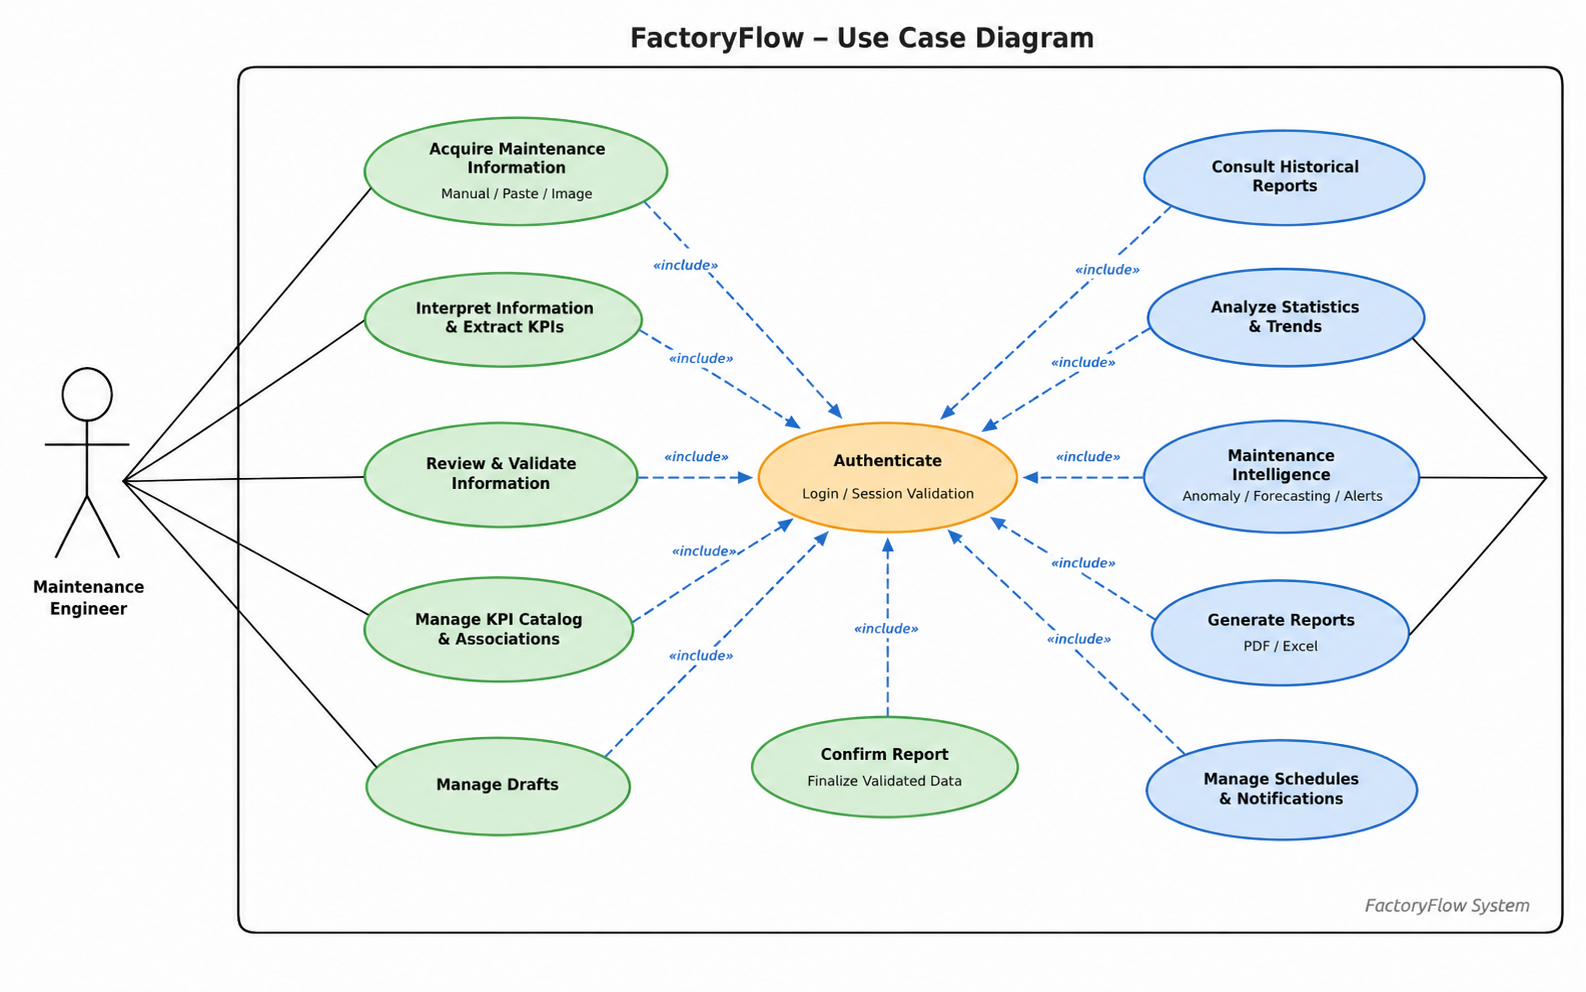
\includegraphics[width=0.98\textwidth]
    {diagrams/source/factoryflow_uc.png}

    \caption{FactoryFlow use case diagram}
    \label{fig:factoryflow-use-case}
\end{figure}

As shown in \textbf{Figure~\ref{fig:factoryflow-use-case}},
authentication is a prerequisite for access to the protected functionalities
of FactoryFlow. The corresponding use case is therefore included by the
principal authenticated operations of the platform.

The Maintenance Engineer can acquire maintenance information through the
supported acquisition mechanisms, review and validate interpreted data,
manage KPI definitions and associations, preserve incomplete work as
drafts, and confirm validated reports.

The same actor can subsequently consult historical information, analyse KPI
statistics and trends, access Maintenance Intelligence results, generate
reports, and manage the scheduling and notification functions associated
with the reporting workflow.

The diagram therefore provides a consolidated representation of the
functional perimeter previously established through the functional
requirements, business rules, and acceptance criteria.


% ============================================================
% CONCLUSION
% ============================================================

% ============================================================
% CONCLUSION
% ============================================================

\section{Conclusion}
\label{sec:requirements-conclusion}

This chapter translated the industrial needs identified in
\textbf{Chapter~\ref{chap:industrial-context}}
into a structured specification for FactoryFlow.

The analysis identified the Maintenance Engineer as the principal human
actor and defined the functional requirements covering acquisition,
deterministic interpretation, human-controlled validation, KPI management,
traceability, historical analysis, reporting, automation, and Maintenance
Intelligence.

The non-functional requirements established the expected levels of data
integrity, reliability, security, usability, maintainability,
interoperability, and analytical reliability. These constraints were
complemented by business rules that preserve the semantic meaning of the
maintenance information, particularly the distinction between missing and
zero values, the management of uncertainty, source traceability, and the
use of validated data for analytical processing.

Finally, the acceptance criteria and UML use case model provided a
verifiable representation of the expected system behaviour and its main
user interactions.

Based on this specification, the next chapter presents the
\textbf{software architecture and detailed design of FactoryFlow},
explaining how these requirements were translated into the technical
components of the platform.